\iffalse
\def\mytitle{MATRIX ANALYSIS USING PYTHON}
\def\myauthor{Soundarya Naru}
\def\contact{narusoundarya2002@gmail.com}
\def\mymodule{Future Wireless Communication (FWC)}
\documentclass[10pt, a4paper]{article}
\usepackage[a4paper,outer=1.5cm,inner=1.5cm,top=1.75cm,bottom=1.5cm]{geometry}
\twocolumn
\usepackage{graphicx}
\graphicspath{{./images/}}
\usepackage[colorlinks,linkcolor={black},citecolor={blue!80!black},urlcolor={blue!80!black}]{hyperref}
\usepackage[parfill]{parskip}
\usepackage{lmodern}
\usepackage{tikz}
\usepackage{physics}
%\documentclass[tikz, border=2mm]{standalone}
%\usepackage{karnaugh-map}
%\documentclass{article}
\usepackage{tabularx}
%\usepackage{circuitikz}
\usepackage{enumitem}
\usetikzlibrary{calc}
\usepackage{amsmath}
\usepackage{amssymb}
\renewcommand*\familydefault{\sfdefault}
\usepackage{watermark}
\usepackage{lipsum}
\usepackage{xcolor}
\usepackage{listings}
\usepackage{float}
\usepackage{titlesec}
\providecommand{\mtx}[1]{\mathbf{#1}}
\titlespacing{\subsection}{1pt}{\parskip}{3pt}
\titlespacing{\subsubsection}{0pt}{\parskip}{-\parskip}
\titlespacing{\paragraph}{0pt}{\parskip}{\parskip}
\providecommand{\qfunc}[1]{\ensuremath{Q\left(#1\right)}}
\providecommand{\sbrak}[1]{\ensuremath{{}\left[#1\right]}}
\providecommand{\lsbrak}[1]{\ensuremath{{}\left[#1\right.}}
\providecommand{\rsbrak}[1]{\ensuremath{{}\left.#1\right]}}
\providecommand{\brak}[1]{\ensuremath{\left(#1\right)}}
\providecommand{\lbrak}[1]{\ensuremath{\left(#1\right.}}
\providecommand{\rbrak}[1]{\ensuremath{\left.#1\right)}}
\providecommand{\cbrak}[1]{\ensuremath{\left\{#1\right\}}}
\providecommand{\lcbrak}[1]{\ensuremath{\left\{#1\right.}}
\providecommand{\rcbrak}[1]{\ensuremath{\left.#1\right\}}}
\newcommand{\figuremacro}[5]{
    \begin{figure}[#1]
        \aligning
        \includegraphics[width=#5\columnwidth]{#2}
        \caption[#3]{\textbf{#3}#4}
        \label{fig:#2}
    \end{figure}
}
\newcommand{\myvec}[1]{\ensuremath{\begin{pmatrix}#1\end{pmatrix}}}
\let\vec\mathbf
\lstset{
frame=single, 
breaklines=true,
columns=fullflexible
}
%\thiswatermark{\aligning \put(181,-119.0){
\includegraphics[scale=0.13]{iith_logo3}} }
\title{\mytitle}
\author{\myauthor\hspace{1em}\\\contact\\FWC22034\hspace{6.5em}IITH\hspace{0.5em}\mymodule\hspace{6em}Assignment}
\begin{document}
	\maketitle
	\tableofcontents
   \section{Problem}
   \fi
 Find points on the curve $\frac{x^2}{9}+\frac{y^2}{16}=1$ at which the tangents are 
 \begin{enumerate}
	 \item parallel to x-axis\\  
	 \item parallel to y-axis
 \end{enumerate}
 \solution 
	\begin{figure}[!h]
		\centering
 \includegraphics[width=\columnwidth]{chapters/12/6/3/13/figs/conic_1.pdf}
		\caption{}
		\label{fig:12/6/3/13}
  	\end{figure}
 \iffalse
\section{Construction}
  \includegraphics[scale=0.5]{conic_1.pdf}
  \begin{align}
  Figure of construction
  	\end{align}
  The dimensions of the figure is taken as below\\\\
{
\setlength\extrarowheight{2pt}
\aligning
\begin{tabular}{|c|c|}
 \hline
 \textbf{Symbol}&\textbf{Value}\\
 \hline
 a&3\\
 \hline
 b&4\\
 \hline
\end{tabular}
}	
  \section{Solution}

Ellipse equation : \begin{align}
\frac{x^2}{9}+\frac{y^2}{16}=1
  \end{align}
The standard equation of the conics is given as :
\begin{align}
\vec{x}^{\top}\vec{V}\vec{x}+2\vec{u}^{\top}\vec{x}+f=0
\end{align}
\fi
The parameters of the given conic are
\begin{align}
	\lambda_1&=16,\lambda_2=9 \\ \vec{V} &= \myvec{	\lambda_1& 0 \\
			          0 & \lambda_2}  
		    , \vec{u} = \myvec{0 \\0}, f = -144
		\label{eq:12/6/3/13/params}
	\end{align}
	\iffalse
	(i) Find points on the curve $\frac{x^2}{9}+\frac{y^2}{16}=1$ at which the tangents are parallel to x-axis\\
	
The points are given by the following equation\\
\begin{equation}
\vec{q}=\vec{v}^{-1}(k_i\vec{n_1}-\vec{u})
\end{equation}
And the intermediate parameters are given by\\
\begin{equation}
k_i=\pm\sqrt{\frac{\vec{u}^T\vec{v}^{-1}\vec{u}-f}{\vec{n_1}^T\vec{v}^{-1}\vec{n_1}}}
\end{equation}
\fi
\begin{enumerate}
	\item The 
normal vector  in this case is
\begin{align}
		\vec{n_1}=\myvec{0\\1}
\end{align}
which can be used along with the parameters in 
		\eqref{eq:12/6/3/13/params}
		to obtain 
\begin{equation}
\vec{q_1}=\myvec{0\\4},
\vec{q_2}=\myvec{0\\-4}
\end{equation}
using 
\eqref{eq:conic_tangent_qk}.
\item Simlarly, 
	choosing
\begin{align}
	\vec{n_2}&=\myvec{1\\0},
	\\
	\vec{q_3}&=\myvec{3\\0},
	\vec{q_4}=\myvec{-3\\0}
\end{align}
\end{enumerate}
\iffalse
Now to obtain the k1 and k2 values substitute n1 value in equation (6)\\
\begin{equation}
\vec{v}^{-1}=\myvec{1/16&0\\0&1/9}
\end{equation}
\begin{equation}
k_1=\sqrt{\frac{\myvec{0\\0}^T\myvec{1/16&0\\0&1/9}\myvec{0\\0}}{\myvec{0\\1}^T\myvec{1/16&0\\0&1/9}\myvec{0\\1}}}
\end{equation}
\begin{equation}
k_1=31.17
\end{equation}
k1 value substitute in equation (5) we get q1\\
\begin{equation}
\vec{q_1}={\myvec{1/16&0\\0&1/9}(k_1\myvec{0\\1}-\myvec{0\\0})}
\end{equation}
\begin{equation}
\vec{q_1}=\myvec{0\\4}
\end{equation}
\begin{equation}
k_2=-\sqrt{\frac{\myvec{0\\0}^T\myvec{1/16&0\\0&1/9}\myvec{0\\0}}{\myvec{0\\1}^T\myvec{1/16&0\\0&1/9}\myvec{0\\1}}}
\end{equation}
\begin{equation}
k_2=-31.17
\end{equation}
k2 value substitute in equation (5) we get q1\\
\begin{equation}
\vec{q_2}={\myvec{1/16&0\\0&1/9}(k_1\myvec{0\\1}-\myvec{0\\0})}
\end{equation}
\begin{equation}
\vec{q_2}=\myvec{0\\-4}
\end{equation}
	(ii) Find points on the curve $\frac{x^2}{9}+\frac{y^2}{16}=1$ at which the tangents are parallel to y-axis\\
	
The points are given by the following equation\\
\begin{equation}
\vec{q}=\vec{v}^{-1}(k_i\vec{n_2}-\vec{u})
\end{equation}
And the intermediate parameters are given by\\
\begin{equation}
k_i=\pm\sqrt{\frac{\vec{u}^T\vec{v}^{-1}\vec{u}-f}{\vec{n_2}^T\vec{v}^{-1}\vec{n_2}}}
\end{equation}
Here $\vec{n_2}$ is normal vector which is parallel to y-axis.\\
\begin{align}
		$\vec{n_2}=\myvec{1\\0}$\\
\end{align}
Now to obtain the k3 and k4 values substitute n2 value in equation (17)\\
\begin{equation}
\vec{v}^{-1}=\myvec{1/16&0\\0&1/9}
\end{equation}
\begin{equation}
k_3=\sqrt{\frac{\myvec{0\\0}^T\myvec{1/16&0\\0&1/9}\myvec{0\\0}}{\myvec{1\\0}^T\myvec{1/16&0\\0&1/9}\myvec{1\\0}}}
\end{equation}
\begin{equation}
k_3=55.42
\end{equation}
k3 value substitute in equation (16) we get q3\\
\begin{equation}
\vec{q_3}={\myvec{1/16&0\\0&1/9}(k_1\myvec{0\\1}-\myvec{0\\0})}
\end{equation}
\begin{equation}
\vec{q_3}=\myvec{3\\0}
\end{equation}
\begin{equation}
k_4=-\sqrt{\frac{\myvec{0\\0}^T\myvec{1/16&0\\0&1/9}\myvec{0\\0}}{\myvec{1\\0}^T\myvec{1/16&0\\0&1/9}\myvec{1\\0}}}
\end{equation}
\begin{equation}
k_4=-31.17
\end{equation}
k4 value substitute in equation (16) we get q1\\
\begin{equation}
\vec{q_4}={\myvec{1/16&0\\0&1/9}(k_1\myvec{1\\0}-\myvec{0\\0})}
\end{equation}
\begin{equation}
\vec{q_4}=\myvec{-3\\0}
\end{equation}
The points on the curve $\frac{x^2}{9}+\frac{y^2}{16}=1$ at which the tangents are parallel to x-axis and parallel to y-axis\\
\begin{equation}
\vec{q_1}=\myvec{0\\4},\vec{q_2}=\myvec{0\\-4}
\end{equation}
\begin{equation}
\vec{q_3}=\myvec{3\\0},\vec{q_4}=\myvec{-3\\0}
\end{equation}
\begin{align}
Below python code realizes the above construction :
\fbox{\parbox{8.5cm}{\url{https://github.com/soundaryanaru/FWC-assignments/blob/main/Matrix/Conic_assignment/code/ellipse.py}}}
\end{align}
\end{document}
\fi
